\input{/home/nick/latex-preambles/xelatex.tex}

\newcommand{\imagesPath}{.}

\title{\textbf{Δίκτυα Υπολογιστών} \\~\\Εργαστηριακή Άσκηση 2 \\ Ενθυλάκωση και Επικεφαλίδες}
\author{}
\date{}

\begin{document}
	\maketitle
	
	\begin{tabular}{|l|l|}
		\hline
		\textbf{Ονοματεπώνυμο:} Νικόλαος Παγώνας, el18175 & \textbf{Ομάδα:} 4 (Τρίτη εξ' αποστάσεως) \\
		\hline
		\textbf{Όνομα PC/ΛΣ:} nick-ubuntu/Ubuntu 20.04.3 LTS & \textbf{Ημερομηνία:} Τρίτη 19/10/2021  \\
		\hline
		\textbf{Διεύθυνση IP:} \verb|192.168.1.15| & \textbf{Διεύθυνση MAC:} \verb|3c:2c:30:e1:1c:55|\\
		\hline
	\end{tabular}

	\subsection*{1. Στρώμα ζεύξης δεδομένων}
		
		\subsubsection*{1.1}
			Με το φίλτρο \verb+arp || ip+ εμφανίζονται μόνο τα πακέτα που έχουν πρωτόκολλο \verb|ARP| ή \verb|IP|.  
		
		\subsubsection*{1.2}
			Τα ονόματα των πεδίων της επικεφαλίδας του πλαισίου Ethernet είναι: \verb|Destination, Source, Type|
		
		\subsubsection*{1.3}
			Όχι, δεν υπάρχει τέτοιο πεδίο.
		
		\subsubsection*{1.4}
			Οι διευθύνσεις Ethernet έχουν μήκος 6 byte.
		
		\subsubsection*{1.5}
			Κάνουμε highlight την επικεφαλίδα Ethernet ώστε να δούμε την αντιστοιχία της σε byte: 
			
			\begin{figure}[H]
				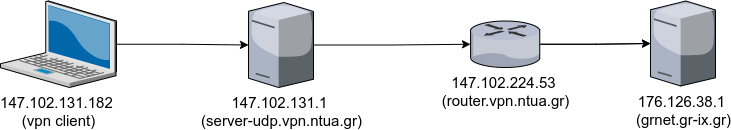
\includegraphics[width=\linewidth]{\imagesPath/1.5.png}
			\end{figure}
		
			Παρατηρούμε λοιπόν ότι το συνολικό μήκος της επικεφαλίδας Ethernet είναι 14 byte.
			
		\subsubsection*{1.6}
		
			Το πεδίο του πλαισίου Ethernet που καθορίζει το πρωτόκολλο δικτύου είναι το πεδίο \verb|Type|.
			
		
		\subsubsection*{1.7}
			
			Η θέση που καταλαμβάνει μέσα στην επικεφαλίδα Ethernet είναι στο τέλος-τέλος (τελευταία δύο bytes), όπως φαίνεται και στην εικόνα: 
			
			\begin{figure}[H]
				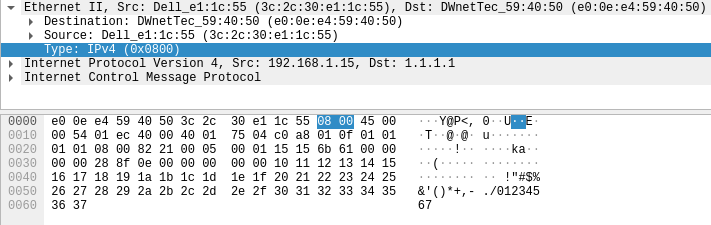
\includegraphics[width=\linewidth]{\imagesPath/1.7.png}
			\end{figure}
		
		\subsubsection*{1.8}
			Η τιμή του πεδίου αυτού για πακέτα IPv4 είναι \verb|0x0800|.
		
		\subsubsection*{1.9}
			Για ARP πακέτα, η τιμή του πεδίου είναι \verb|0x0806|.
	
	\subsection*{2. Στρώμα Δικτύου}
		
		\subsubsection*{2.1}
			Το φίλτρο \verb|icmp| εμφανίζει μόνο πακέτα που έχουν πρωτόκολλο ICMP.
		
		\subsubsection*{2.2}
			Το μήκος των διευθύνσεων IPv4 είναι 4 bytes.
		
		\subsubsection*{2.3}
			Τα ονόματα των δύο πρώτων πεδίων της επικεφαλίδας IPv4 είναι \verb|Version| και \verb|Header Length|.
		
		\subsubsection*{2.4}
			Το μήκος σε bit τόσο του πεδίου \verb|Version| όσο και του πεδίου \verb|Header Length| είναι 4 bit (όπως φαίνεται από τον σύνδεσμο που παρατίθεται στην εκφώνηση της αναφοράς, αλλά και από το \verb|Wireshark|). \\
			Η τιμή του πεδίου Version είναι \textbf{0100} (Version 4), ενώ του πεδίου Header Length είναι \textbf{0101}, που αντιστοιχεί σε 20 bytes, όπως αναγράφεται και στο Wireshark.
		
		\subsubsection*{2.5}
		
			Στο Wireshark, κάνουμε highlight την επικεφαλίδα IPv4 και βλέπουμε ότι έχει συνολικό μέγεθος 20 bytes.
			
			\begin{figure}[H]
				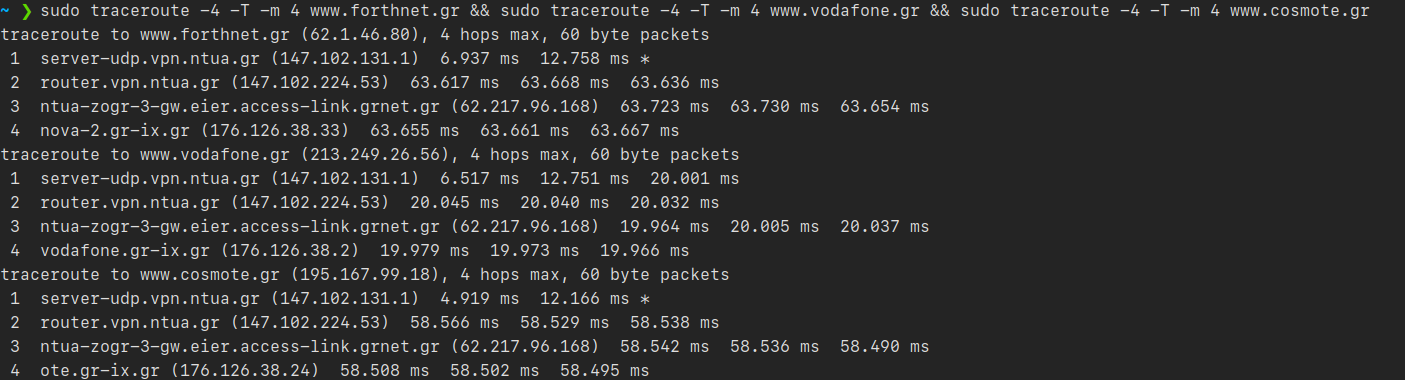
\includegraphics[width=\linewidth]{\imagesPath/2.5.png}
			\end{figure}
		
		\subsubsection*{2.6}
			
			Από το site που παρατέθηκε στην εκφώνηση σχετικά με το πρωτόκολλο IPv4:
			
			\begin{figure}[H]
				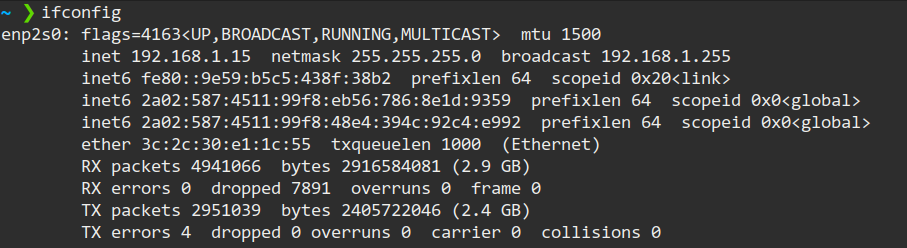
\includegraphics[width=\linewidth]{\imagesPath/2.6.png}
			\end{figure}
		
			Αυτό σημαίνει ότι αφού το Header Length έχει τιμή 5, τότε η επικεφαλίδα έχει μέγεθος: 
				\[
					\dfrac{5 \cdot 32}{8} = 20 \text{ bytes.}
				\]
				
			Με αυτόν τον τρόπο λοιπόν προκύπτει και το μέγεθος της επικεφαλίδας, χωρίς να χρειαστούμε τη βοήθεια του παραθύρου περιεχομένων.
			
		\subsubsection*{2.7}
			Βλέπουμε από το παράθυρο με τα περιεχόμενα ότι το συνολικό μήκος αυτού του πακέτου είναι 84 bytes.
		
		\subsubsection*{2.8}
			Υπάρχει το πεδίο \verb|Total Length| με τιμή 84 bytes, η οποία συμφωνεί με το παραπάνω.
		
		\subsubsection*{2.9}
			Το μήκος δεδομένων του πακέτου IPv4 είναι 64 bytes.
			
		
		\subsubsection*{2.10}
			Το μήκος των δεδομένων προκύπτει αν από το \verb|Total Length| αφαιρέσουμε το \verb|Header Length|: 
				\[
					(84 - 20 = 64 \text{ bytes})
				\]
		
		\subsubsection*{2.11}
			Το πεδίο που καθορίζει το πρωτόκολλο στρώματος μεταφοράς είναι το \verb|Protocol|.
		
		\subsubsection*{2.12}
			Η θέση του σε σχέση με την αρχή της επικεφαλίδας IPv4 είναι στο 10$^{\text{ο}}$ byte.
		
		\subsubsection*{2.13}
			Για το πρωτόκολλο ICMP η τιμή του είναι 01.
		
	\subsection*{3. Στρώμα Μεταφοράς}
		
		\subsubsection*{3.1}
			Το παραπάνω φίλτρο απεικόνισης εμφανίζει μόνο πακέτα που έχουν πρωτόκολλο \verb|TCP| ή \verb|UDP|.
		
		\subsubsection*{3.2} 
			Παρατηρούμε τα πρωτόκολλα \verb|TCP| και \verb|UDP|.
		
		\subsubsection*{3.3}
			Η τιμή του πεδίου \verb|Protocol| στην επικεφαλίδα IPv4 για το πρωτόκολλο TCP είναι 6, ενώ για το UDP είναι 17 (στο δεκαδικό σύστημα).
		
		\subsubsection*{3.4}
			Τα κοινά ονόματα πεδίων μεταξύ των δύο πρωτοκόλλων είναι: \verb|Source Port, Destination Port| και \verb|Checksum|.
					
		\subsubsection*{3.5}
			Το μήκος της επικεφαλίδας των δεδομενογραμμάτων UDP είναι 8 bytes.
		
		\subsubsection*{3.6}
			Ναι, υπάρχει (το πεδίο \verb|Length|).
		
		\subsubsection*{3.7}
			Το πεδίο που καθορίζει το μήκος της επικεφαλίδας του τεμαχίου TCP είναι το \verb|Header Length|, και βρίσκεται στο 13$^{\text{ο}}$ byte της επικεφαλίδας (συγκεκριμένα στα 4 MSB).
		
		\subsubsection*{3.8}
			Δεν υπάρχει πεδίο που να δίνει το συνολικό μήκος ενός τεμαχίου TCP. Το μήκος αυτό προκύπτει ως εξής: 
			
			\[
				\text{Μήκος πλαισίου IP} - (\text{Μήκος επικεφαλίδας IP} + \text{Μήκος επικεφαλίδας TCP})
			\]
		
			Μπορούμε να βρούμε το μήκος πλαισίου IP από το πεδίο \verb|Total Length| του IP header, το μήκος επικεφαλίδας IP από το πεδίο \verb|Header Length|, και το μήκος επικεφαλίδας TCP από το πεδίο \verb|Header Length| του TCP header.

		\subsubsection*{3.9}
			Με βάση το \verb|Destination Port| του TCP header μπορούμε να βρούμε τον τύπο του πρωτοκόλλου εφαρμογής, αντιστοιχώντας το εκάστοτε port, με τη βοήθεια του πίνακα που βρίσκεται στο link της εκφώνησης.
		
		\subsubsection*{3.10}
			Άλλα πρωτόκολλα εφαρμογής που παρατηρήθηκαν στον πίνακα είναι:
			\begin{itemize}
				\item RWP, Remote Write Protocol
				\item FTP, File Transfer Protocol 
				\item SMTP, Simple Mail Transfer Protocol
				\item RAP, Internet Route Access Protocol
				\item Internet Message Protocol
				\item MTP, Mail Transfer Protocol
			\end{itemize}
	\subsection*{4. Στρώμα Εφαρμογής}
		
		\subsubsection*{4.1}
			To \verb|DNS| χρησιμοποιεί το πρωτόκολλο \verb|UDP|.
		
		\subsubsection*{4.2}
			Tο \verb|HTTP| χρησιμοποιεί το πρωτόκολλο \verb|TCP|.
			
		
		\subsubsection*{4.3}
			Όπως βλέπουμε στο λινκ που παρατέθηκε στην εκφώνηση (αλλά και στο Wireshark), το πρώτο bit της σημαίας μας δείχνει αν πρόκειται για ερώτηση (οπότε θα είναι 0) ή για απάντηση (οπότε θα είναι 1).
		
		\subsubsection*{4.4}
			Η θύρα προορισμού των ερωτήσεων DNS είναι η 53.
		
		\subsubsection*{4.5}
			Αντίστοιχα, οι θύρες προέλευσης των ερωτήσεων DNS είναι οι 34512, 33415, 35278, 41535, 34401, 48900, 45347, 57290, 56403, 58318.
			
		
		\subsubsection*{4.6}
			Η θύρα προέλευσης των απαντήσεων DNS είναι πάλι η 53.
		
		\subsubsection*{4.7}
			Οι θύρες προορισμού των απαντήσεων DNS είναι οι 34512, 33415, 35278, 41535, 34401, 48900, 45347, 57290, 56403, 58318. 
		
		\subsubsection*{4.8}
			Οι θύρες προορισμού των απαντήσεων είναι ίδιες με τις θύρες προέλευσης των ερωτήσεων DNS που βρήκαμε πριν, και με ίδια σειρά. Αυτό είναι λογικό, αφού η θύρα στην οποία γίνεται μία ερώτηση θα πρέπει να είναι και η θύρα στην οποία θα δοθεί η απάντηση.
		
		\subsubsection*{4.9}
			Η well-known θύρα όπου ακούει ο εξυπηρετητής DNS είναι η 53.
		
		\subsubsection*{4.10}
			Η θύρα προορισμού των μηνυμάτων HTTP που παράγει ο υπολογιστής μας είναι η θύρα 80.
		
		\subsubsection*{4.11}
			Η θύρα προέλευσης των μηνυμάτων HTTP που έστειλε ο υπολογιστής μας είναι η 42994.
		
		\subsubsection*{4.12}
			Η θύρα προέλευσης των αντίστοιχων απαντήσεων HTTP του εξυπηρετητή ιστού είναι η 80.
		
		\subsubsection*{4.13}
			Η θύρα προορισμού των απαντήσεων είναι η 42994.
		
		\subsubsection*{4.14}
			Η well-known θύρα όπου ακούει ο εξυπηρετητής HTTP είναι η 80.
	
		\subsubsection*{4.15}
			Παρατηρούμε ότι οι θύρες προέλευσης των μηνυμάτων HTTP είναι ίδιες με τις θύρες προορισμού των αντίστοιχων απαντήσεων του εξυπηρετητή. Αυτό είναι λογικό, αφού η θύρα στην οποία γίνεται μία ερώτηση θα πρέπει να είναι και η θύρα στην οποία θα δοθεί η απάντηση.
		
		\subsubsection*{4.16}
			Η ονομασία του πρώτου μηνύματος HTTP από τον υπολογιστή μας προς τον server είναι: \\
			\verb|GET /lab2/ HTTP/1.1 .|
		
		\subsubsection*{4.17}
			Η απάντηση είναι: \verb|HTTP/1.1 200 OK| άρα ο κωδικός είναι 200 OK.
		
		\subsubsection*{4.18}
			Βλέπουμε ότι αν ξαναεπισκεφτούμε την ιστοσελίδα, δεν καταγράφεται κίνηση πακέτων με πρωτόκολλο DNS, αφού οι αντιστοιχίσεις υπάρχουν αποθηκευμένες από πριν και άρα δεν χρειάζεται να ξαναγίνει η αντιστοίχιση. Εκτελώντας την εντολή \verb|sudo systemd-resolve --flush-caches|, σιγουρεύουμε ότι θα σταλούν και αυτά τα πακέτα.

\end{document}